\documentclass[justified,notoc,openany]{tufte-book}

% --- Encoding and fonts ---
\usepackage[utf8]{inputenc}
\usepackage[T1]{fontenc}
\usepackage{textcomp}

% --- Graphics ---
\usepackage{graphicx}
\graphicspath{
  {../}
  {../CM3070-Models-Implementation-Evaluation/reports/figures/}
  {../CM3070-Model-Serving-Triton-ONNX/accessibility_evidence/}
}

% --- Tables ---
\usepackage{booktabs}
\usepackage{tabularx}

% --- Math ---
\usepackage{amsmath}
\usepackage{amssymb}

% --- Colors (before hyperref setup) ---
\usepackage{xcolor}

% --- URL line-breaking (must load before hypersetup) ---
\usepackage{xurl}

% --- Hyperlinks (tufte-book loads hyperref, just configure it) ---
\hypersetup{
  colorlinks=true,
  linkcolor=darkgray,
  citecolor=darkgray,
  urlcolor=blue!60!black,
  pdfauthor={David Cardozo},
  pdftitle={Design and Evaluation of a Modular Deep Learning Pipeline for Mammography-Based Breast Cancer Patch Classification}
}

% --- Bibliography style (tufte-book loads natbib) ---
\bibliographystyle{plainnat}

% --- Code listings ---
\usepackage{listings}
\lstset{
  basicstyle=\ttfamily\small,
  breaklines=true,
  frame=single,
  framesep=3pt,
  framexleftmargin=3pt,
  backgroundcolor=\color{gray!10}
}

% --- Allow hyphenation in monospace (\texttt) ---
\usepackage[htt]{hyphenat}

% --- Micro-typography ---
\usepackage{microtype}

% --- Tighter lists ---
\providecommand{\tightlist}{%
  \setlength{\itemsep}{0pt}\setlength{\parskip}{0pt}}

% --- Allow longtable from pandoc to work ---
\usepackage{longtable}

% --- Non-floating captions ---
\usepackage{caption}

% --- Include external PDF pages (for cover) ---
\usepackage{pdfpages}

% --- "This page intentionally left blank" on empty pages ---
\makeatletter
\def\cleardoublepage{\clearpage\if@twoside \ifodd\c@page\else
  \hbox{}
  \vfill
  \begin{center}
    \textit{This page intentionally left blank.}
  \end{center}
  \vfill
  \thispagestyle{empty}
  \newpage
  \if@twocolumn\hbox{}\newpage\fi\fi\fi}
\makeatother

% --- Title data ---
\title{Design and Evaluation of a Modular Deep Learning Pipeline for Mammography-Based Breast Cancer Patch Classification}
\author{David Cardozo}
\date{2026-03-21}

\begin{document}

% --- Don't stretch vertical space to fill pages ---
\raggedbottom

% --- Cover page from external PDF ---

\includepdf[pages=1]{cover-thesis/cover.pdf}

% --- Table of contents ---
\tableofcontents

\chapter{Introduction (883/1000 words)}\label{introduction-8831000-words}

This project follows \textbf{template 3.2 Project Idea 2: Deep Learning Breast Cancer Detection}.

\section{Background}\label{background}

Breast cancer is the leading cause of cancer-related mortality among women in Colombia, with an estimated 17,018 new cases and 4,752 deaths annually \cite{ValbuenaGarcia2025}. Early-Onset Breast Cancer (EOBC), diagnosed in women aged 18 to 45, accounts for approximately 19.4\% of cases in the country. These cases are often more aggressive, presenting significant clinical challenges due to late-stage diagnosis and systemic delays in treatment initiation that frequently exceed 60 days \cite{ValbuenaGarcia2025}. Medical imaging techniques, particularly X-ray mammography, serve as the gold standard for breast cancer screening due to their ability to detect abnormalities such as lumps, calcifications, and tissue distortions. However, mammography has inherent limitations, including reduced sensitivity in women with dense breast tissue and significant variability in interpretation among radiologists \cite{Wang2024}.

Computer-assisted detection and diagnosis (CAD) systems have been in clinical use since the 1990s, yet empirical evidence suggests that commercial CAD systems have not delivered significant performance improvements, with reported average AUC values of approximately 0.72 \cite{Carriero2024}. According to the Breast Cancer Surveillance Consortium, the overall sensitivity of digital screening mammography in the United States stands at 84.4\% with a specificity of 90.8\%, indicating substantial room for improvement in reducing both false positives and false negatives \cite{Carriero2024}. These challenges have motivated extensive research into deep learning approaches that can enhance diagnostic accuracy and consistency in breast cancer detection.

\section{Motivation}\label{motivation}

This project is motivated by three key needs. First, there is a pressing need for scalable and reproducible data pipelines that can transform raw mammographic imaging data into model-ready formats while maintaining full traceability of each processing step. Existing approaches to working with medical imaging datasets frequently rely on ad hoc acquisition practices, informal preprocessing scripts, and repackaged dataset copies from secondary platforms such as Kaggle. This lack of reproducibility undermines the reliability of downstream modelling and makes it difficult for other researchers to verify or extend published results.

Second, the field requires a systematic comparative understanding of model architectures across the full spectrum from classical machine learning to modern deep learning. While individual studies routinely report state-of-the-art results for specific architectures, there are relatively few end-to-end comparisons that evaluate classical baselines, convolutional networks trained from scratch, and pretrained transformer models within a single experimental framework using identical data and consistent evaluation metrics. Such a comparison is essential for understanding the relative contributions of feature engineering, model capacity, and transfer learning to classification performance, and for guiding practical decisions about which approaches to deploy in resource-constrained environments.

Third, clinical trust in automated diagnostic tools depends fundamentally on model explainability. Healthcare professionals require transparent decision-making processes to validate AI-assisted predictions and to identify potential failure modes before clinical adoption \cite{Lee2017}. Explainability techniques that produce visual heatmaps highlighting diagnostically relevant regions offer a natural interface for radiologists, who are already trained to interpret spatial patterns in mammographic images.

\section{Project Concept and Contributions}\label{project-concept-and-contributions}

This project implements an end-to-end pipeline for breast cancer patch classification on the Curated Breast Imaging Subset of the Digital Database for Screening Mammography (CBIS-DDSM). The pipeline is organized as a modular, multi-repository collection with six stages: data acquisition from the National Biomedical Imaging Archive (NBIA), distributed DICOM-to-PNG conversion on Google Cloud, dataset validation with TensorFlow Data Validation, exploratory data analysis with FiftyOne and embedding-based visualizations, model training and evaluation across three modelling paradigms, and model serving with NVIDIA Triton Inference Server behind an accessible web frontend.

The modelling stage compares three families of approaches: classical machine learning baselines using hand-crafted features (PCA, HOG) with scikit-learn classifiers, deep learning models trained from random initialization on TPU using JAX and Flax, and pretrained models fine-tuned on GPU using PyTorch and the timm library with Grad-CAM explainability. The best-performing model is exported to ONNX format and deployed via Triton on Google Cloud Run with GPU support.

The project makes the following practical contributions. It modernizes the technical stack used to acquire and process the CBIS-DDSM dataset, replacing informal acquisition practices with a reproducible containerized workflow. It provides a correct and efficient pathway for downloading the source data directly from NBIA, rather than relying on repackaged copies from secondary platforms. It establishes a scalable pipeline for converting raw DICOM files into standardized TensorFlow Datasets format that can be consumed consistently by downstream workflows. And it organizes the full process from downloading through deployment into a single repository collection designed for reproducibility and independent verification.

\section{Research Questions}\label{research-questions}

This project is guided by the following research questions:

\begin{enumerate}
\def\labelenumi{\arabic{enumi}.}
\tightlist
\item
  What level of performance can be achieved using classical linear baselines on the curated CBIS-DDSM patch classification task?
\item
  How much improvement is obtained when replacing linear baselines with deep learning models trained from scratch?
\item
  Do pretrained timm models provide a further performance advantage over from-scratch deep learning approaches?
\end{enumerate}

These questions are structured progressively: the first establishes a performance floor using traditional methods, the second quantifies the benefit of learned feature representations, and the third isolates the contribution of transfer learning from ImageNet pretraining.

The preliminary proposal for this project envisioned a Kubeflow-based MLOps pipeline on Vertex AI with VisualBackProp explainability. During implementation, the design evolved toward a modular containerized architecture using Google Cloud Batch and Cloud Build, and GradCAM-based explainability via the pytorch-grad-cam library, which offered superior maturity and broader ecosystem support for the research questions being pursued.

\textbf{Code repository:} \url{https://github.com/Davidnet/CM3070-Thesis-University-curated_breast_imaging_ddsm}

\newpage

\chapter{Literature Review (2326/2500 words)}\label{literature-review-23262500-words}

\section{Deep Learning in Medical Imaging}\label{deep-learning-in-medical-imaging}

Deep learning represents a subset of artificial intelligence techniques that employs multi-layered neural networks to learn hierarchical feature representations directly from data \cite{LeCun1998}. Unlike traditional machine learning approaches that require manually engineered features, deep learning models learn to extract increasingly abstract and task-relevant features through successive layers of nonlinear transformations. In medical imaging, these capabilities have been applied to a wide range of tasks including image classification, object detection, segmentation, and image enhancement \cite{Carriero2024}.

The most common applications of deep learning in medical imaging involve processing images to either infer diagnostic outputs, such as the presence of abnormal findings or the classification of lesion types, or to manipulate image characteristics through noise reduction and spatial resolution enhancement. Convolutional neural networks (CNNs) have shown particularly promising results in mammography applications, with several studies reporting classification accuracy that matches or exceeds that of experienced radiologists. CNN-based mammography systems can achieve area under the curve (AUC) values above 0.84 for breast cancer risk classification \cite{Wang2024,Lotter2021}, often with lower false-positive rates than human experts. Lotter et al.~\cite{Lotter2021} demonstrated that an annotation-efficient deep learning approach could achieve robust breast cancer detection across both standard mammography and digital breast tomosynthesis. However, a critical caveat applies when interpreting these headline results: the majority of published AUC figures are for binary whole-image classification (cancer versus no-cancer), not for the multi-class patch-level task addressed in this project. Whole-image classification benefits from contextual information across the full breast, whereas patch-level classification must distinguish lesion subtypes from a 224 by 224 crop alone, making the tasks fundamentally different in difficulty and limiting the direct comparability of reported metrics.

\section{Mammography-Based Breast Cancer Detection}\label{mammography-based-breast-cancer-detection}

The computational analysis of mammographic imaging has undergone a profound transformation throughout 2024 and 2025, driven by the integration of large-scale foundation models, hybrid transformer architectures, and selective state-space models (SSMs) \cite{Bayatmakou2025}. The Curated Breast Imaging Subset of the Digital Database for Screening Mammography (CBIS-DDSM) remains the preeminent benchmark for verifying the robustness of these architectures, primarily due to its challenging noise profile inherent to digitized screen-film mammography (SFM). While modern clinical environments have largely transitioned to Full-Field Digital Mammography (FFDM) \cite{SawyerLee2016}, the CBIS-DDSM serves as a stress test for deep learning models, revealing vulnerabilities in domain adaptation and feature extraction that cleaner datasets often mask. This strength is also a limitation: models validated exclusively on CBIS-DDSM may not generalize to FFDM data encountered in contemporary clinical practice, and the noise characteristics of digitized film can introduce artefacts that are absent from modern imaging, potentially inflating or deflating performance estimates depending on the architecture.

Early detection of subclinical breast cancer on screening mammography presents a formidable image classification challenge, as malignant regions typically occupy only a small fraction of the total breast image. A typical FFDM image measures approximately 4000 by 3000 pixels, while a cancerous region of interest (ROI) may span as little as 100 by 100 pixels \cite{Carriero2024}. This extreme scale disparity has historically necessitated approaches that require pixel-level ROI annotations, limiting the applicability of deep learning methods to the few public mammography databases with such detailed annotations \cite{Lee2017,Carriero2024}.

The transition from traditional CAD to deep learning approaches has yielded promising results. Shen \cite{Shen2017} developed an end-to-end training methodology that addresses the scarcity of annotated mammography data by leveraging ROI annotations only in the initial training stage, with subsequent stages requiring only image-level cancer status labels. The all-convolutional network architecture achieved a per-image AUC of 0.88 on the CBIS-DDSM test set using a single model, improving to 0.91 with four-model averaging. When transferred to the INbreast FFDM dataset, the same approach achieved an AUC of 0.95 for single models and 0.98 with model averaging \cite{Shen2017}.

A critical finding from recent research concerns the transferability of models across heterogeneous mammography platforms. The intensity profiles between digitized film mammograms and modern FFDM images differ substantially, yet end-to-end trained classifiers can be successfully fine-tuned using remarkably small datasets. With as few as 20 patients (79 images), transfer learning achieved AUCs between 0.87 and 0.92, suggesting that the primary learning challenge lies in recognizing lesion morphology and texture rather than adapting to different intensity distributions \cite{Carriero2024}. This finding is encouraging for transfer learning but should be interpreted cautiously: the reported AUCs are for whole-image binary detection, and it is unclear whether the same degree of transferability holds for fine-grained multi-class patch classification, where the visual differences between benign and malignant subtypes are more subtle than the cancer-versus-normal distinction.

\section{Model Architectures for Medical Image Classification}\label{model-architectures-for-medical-image-classification}

The architectural choices for mammography classification have evolved considerably. Comparative studies between VGG16 and ResNet50 architectures reveal important trade-offs: while VGG-based classifiers offer a smaller parameter footprint (approximately 15 million versus 24 million parameters), they exhibit greater susceptibility to overfitting and require longer training times. ResNet architectures \cite{He2016} benefit from skip connections and batch normalization, enabling faster convergence and better generalization. The residual learning framework addresses the degradation problem observed in very deep networks, where adding more layers can paradoxically increase training error. By learning residual mappings through shortcut connections, ResNets enable the training of substantially deeper networks while maintaining gradient flow. In the context of mammography, ResNets have become a standard backbone architecture, with ResNet50 frequently serving as the default choice for both from-scratch training and transfer learning experiments due to its balance of depth, parameter efficiency, and well-understood training dynamics.

More recent work has extended these findings to Vision Transformers (ViTs) \cite{Dosovitskiy2021}, which leverage self-attention mechanisms to capture long-range dependencies within images. Unlike CNNs, which process local regions through convolutional filters, ViTs divide the input image into fixed-size patches and process the resulting sequence of patch embeddings through transformer layers. This design captures global context from the earliest layers but lacks the translation-equivariant inductive biases that convolutions provide, making ViTs data-hungry and potentially less effective on smaller datasets when trained from scratch. Dosovitskiy et al.~demonstrated that ViTs require substantially larger training datasets than CNNs to achieve competitive performance without pretraining, a limitation that is particularly relevant in medical imaging where labelled data is often scarce. This creates a tension in the literature: ViTs are praised for their ability to capture global context, but the datasets on which they demonstrate this advantage (ImageNet, JFT-300M) are orders of magnitude larger than typical medical imaging benchmarks. Whether the self-attention mechanism offers any advantage on a dataset of approximately 50,000 training patches --- the scale of CBIS-DDSM --- when trained from scratch is an open question that the present project directly investigates.

The Swin Transformer \cite{Liu2021} addresses several limitations of vanilla ViTs by introducing a hierarchical architecture with shifted windows. By computing self-attention within non-overlapping local windows and shifting the window partition between consecutive layers, the Swin Transformer achieves strong performance while maintaining linear computational complexity with respect to image size. This hierarchical design produces multi-scale feature representations similar to those generated by CNNs, making it more suitable for dense prediction tasks and more practical for high-resolution medical imaging applications. The shifted window mechanism also introduces a form of local connectivity that partially compensates for the absence of convolutional inductive biases, potentially making Swin Transformers more amenable to fine-tuning on smaller target datasets.

Transfer learning from ImageNet has become a dominant strategy in medical image classification. Raghu et al.~\cite{Raghu2019} systematically investigated transfer learning for medical imaging and found that even features learned from natural images transfer well to medical tasks when target data is limited, often outperforming models trained from scratch by substantial margins. Their study revealed that the benefits of transfer learning are concentrated primarily in the early and middle layers of the network, where general-purpose features such as edge detectors and texture analysers are learned. The later, more task-specific layers are largely relearned during fine-tuning, but the pretrained initialization provides a significantly better starting point for optimization. Importantly, Raghu et al.~also found that smaller models trained from scratch can sometimes match larger pretrained models when sufficient target data is available, which complicates the simple narrative that pretraining universally dominates. This finding motivates the present project's explicit comparison of from-scratch and pretrained approaches on the same dataset, rather than assuming the superiority of either strategy. The timm library \cite{Wightman2019} provides a comprehensive, well-maintained collection of pretrained image models in PyTorch, enabling systematic comparison of architectures with standardized training recipes, consistent data augmentation pipelines, and reliable weight loading procedures. Its broad coverage of both convolutional and transformer architectures makes it a practical foundation for multi-architecture comparison studies such as this project.

For classical machine learning, dimensionality reduction techniques such as PCA and feature descriptors such as Histogram of Oriented Gradients (HOG) remain relevant as baselines in medical imaging research, establishing performance floors against which deep learning approaches can be measured. HOG descriptors, originally developed for pedestrian detection, encode local gradient orientation distributions that can capture edge and texture information relevant to lesion morphology, while PCA provides a compact representation of the dominant variance modes in the image space. Gradient-boosted tree ensembles such as HistGradient-Boosting have been shown to perform competitively on tabular representations of image features, particularly when combined with dimensionality reduction, because they can model nonlinear decision boundaries without requiring the large datasets needed by deep learning models.

\section{Explainability Methods}\label{explainability-methods}

Despite strong classification performance, most existing deep learning approaches provide limited transparency into their decision-making processes. The lack of explainability remains a significant barrier to clinical adoption, particularly in high-stakes diagnostic contexts where radiologists must be able to interpret and validate automated predictions \cite{Lee2017}. The literature emphasizes the importance of visual interpretability methods but offers limited integration of such techniques into modern training and deployment pipelines.

Gradient-weighted Class Activation Mapping (GradCAM) \cite{Selvaraju2017} computes a weighted combination of feature map activations at a target layer, where the weights are the gradients of the target class score with respect to each feature map channel, averaged spatially. The resulting weighted sum is passed through a ReLU to produce coarse heatmaps that highlight broad regions of interest. GradCAM is architecture-agnostic and can be applied to any CNN or transformer with a spatially structured feature representation.

HiResCAM \cite{DraelosCarin2021} replaces the spatial averaging of gradients with element-wise multiplication of gradients and activations, preserving spatial resolution and yielding sharper, more localized heatmaps that better delineate fine-grained structures. Draelos and Carin argue that this modification produces more faithful explanations that better reflect the model's actual computation, particularly for architectures where spatial averaging can obscure localized features.

EigenCAM \cite{MuhammadYeasin2020} extracts the first principal component of the feature map activations without using gradient information, producing class-agnostic but structurally coherent heatmaps. Because it relies on the dominant activation mode rather than class-specific gradients, EigenCAM captures the most salient spatial features regardless of the target class. These three methods are implemented in the pytorch-grad-cam library, which provides a unified interface for applying multiple CAM techniques across diverse architectures. However, a broader limitation of all CAM-based methods is that they approximate the model's internal reasoning rather than faithfully representing it; Draelos and Carin's argument for HiResCAM implicitly acknowledges that GradCAM's spatial averaging can produce misleading explanations. The fact that different methods highlight different regions for the same prediction underscores that these are interpretive tools with varying degrees of faithfulness, not ground-truth explanations of model behaviour. For patch-level mammography classification in particular, where diagnostically relevant features may be smaller than the spatial resolution of the CAM output, this limitation is especially relevant.

\section{Deployment and Serving Infrastructure}\label{deployment-and-serving-infrastructure}

The successful translation of deep learning models to clinical practice depends on deployment infrastructure that supports reproducibility, versioning, and maintainability \cite{Grant2020}. The Open Neural Network Exchange (ONNX) format \cite{ONNX2019} provides a framework-agnostic model representation, decoupling training from deployment and enabling interoperability between frameworks such as PyTorch and specialized inference runtimes. NVIDIA Triton Inference Server \cite{NVIDIA2025} serves as an optimized runtime supporting multiple model formats, dynamic batching, and model versioning, suitable for production scenarios where latency and throughput must be managed.

Containerization through Docker and orchestration through cloud-native services such as Google Cloud Build and Cloud Batch provide the foundation for reproducible ML pipelines \cite{Grant2020}. Declarative configuration files ensure that infrastructure is version-controlled alongside code, supporting auditability across pipeline executions \cite{Bradbury2018}.

\section{Web Accessibility in Clinical Tools}\label{web-accessibility-in-clinical-tools}

Clinical decision-support tools must be accessible to the broadest possible range of healthcare professionals, including those who rely on assistive technologies such as screen readers, keyboard-only navigation, or reduced-motion displays. The Web Content Accessibility Guidelines (WCAG) \cite{W3C2018} establish a comprehensive framework for making web content perceivable, operable, understandable, and robust. In medical web applications, ARIA (Accessible Rich Internet Applications) live regions enable screen readers to announce dynamic content updates such as inference results, classification confidence scores, and error messages without requiring user-initiated page navigation. Semantic HTML and keyboard navigation patterns ensure that interactive elements remain operable without a mouse, which is particularly important in clinical environments where assistive technology use may be more common than in general consumer applications. The adoption of accessibility standards in clinical AI interfaces supports inclusive design and aligns with the operational realities of diverse healthcare environments, including the resource-constrained settings that motivate this project.

\section{Ethical Considerations}\label{ethical-considerations}

This project relies exclusively on the CBIS-DDSM dataset, a publicly available, de-identified mammography collection hosted by The Cancer Imaging Archive (TCIA), originally collected under IRB approval and fully anonymized in compliance with HIPAA Safe Harbor provisions \cite{Lee2017,Clark2013}. The model outputs are intended as research demonstrations and are not suitable for clinical diagnosis without further validation.

\section{Synthesis and Experimental Design Rationale}\label{synthesis-and-experimental-design-rationale}

The literature presents several competing claims that this project is designed to resolve empirically. Raghu et al.~\cite{Raghu2019} suggest that from-scratch training can sometimes match pretrained models given sufficient data, while the broader transfer learning literature treats pretraining as universally beneficial. Dosovitskiy et al.~\cite{Dosovitskiy2021} demonstrate that ViTs are data-hungry without pretraining, but it is unclear whether this disadvantage persists at the scale of CBIS-DDSM (\textasciitilde50,000 patches). Most published CBIS-DDSM results report whole-image binary AUC \cite{Shen2017}, leaving the difficulty of multi-class patch classification largely uncharacterised. This project directly tests these tensions by training identical architecture families (ResNet, ViT/Swin) both from scratch and from pretrained weights on the same dataset, using consistent metrics and cross-task alignment to enable comparison across all three modelling paradigms.

\newpage

\chapter{Design (1578/2000 words)}\label{design-15782000-words}

\section{Domain and Users}\label{domain-and-users}

The domain of this project lies at the intersection of diagnostic radiology, oncology, and machine learning infrastructure for resource-constrained healthcare environments. While the primary medical focus is the early detection of breast cancer via mammography, the operational domain addresses the specific infrastructural challenges of deploying artificial intelligence in developing nations. The project operates within the context of the Colombian healthcare system, a setting where advanced diagnostic expertise is concentrated in major urban centres while peripheral regions often face significant delays in diagnosis and treatment initiation. This domain is defined by a critical tension: the need for state-of-the-art diagnostic accuracy, comparable to that of large research hospitals, versus the reality of limited computational infrastructure and the prevalence of aggressive Early-Onset Breast Cancer phenotypes.

Within this domain, the system is designed to serve two distinct user groups. Clinical radiologists, the primary end-users, are responsible for interpreting screening mammograms and making final diagnostic decisions. They are not expected to have expertise in deep learning; their interaction with the system is centred on trust and utility rather than technical configuration. They require a tool that provides not only probability scores but visual justification for predictions, allowing them to validate and contextualize AI-assisted findings within their existing diagnostic workflows. Healthcare IT and MLOps engineers, the technical users, are responsible for maintaining hospital information systems and ensuring the continuous validity of diagnostic tools. They require a reproducible, scalable framework that can be updated as patient demographics shift or new imaging hardware is acquired, without requiring a complete re-architecting of the system.

\section{System Architecture}\label{system-architecture}

The project is organized as a meta-repository containing six primary submodules, with three additional nested submodules for the modelling stage. Each stage is independently containerized, version-controlled, and environment-managed using \texttt{uv} as the Python package manager. This modular design ensures that each component can be developed, tested, and deployed independently while maintaining reproducibility through explicit submodule version pinning. The separation of concerns allows stages to be executed locally, on hyperscaler infrastructure, or in other cloud environments, provided the required dependencies and resources are available.

The separation between stages is important not only for modularity but also for operational independence. Cloud Build answers ``how do I package each stage's environment?'' while Cloud Batch answers ``where and with what machine do I run that packaged environment?'' This separation enables each stage to be executed independently, cached, and re-run without affecting other stages, which is essential for iterative development where model training may be repeated many times while the data preparation stages remain stable.

\textbf{Stage 1 -- Data Acquisition.} The \texttt{CM3070-Downloader} repository packages the NBIA Data Retriever CLI in a multi-stage Docker build. The first stage compiles the Go-based retrieval binary from source, and the second stage copies the compiled binary alongside a bundled CBIS-DDSM manifest into a minimal runtime image. Google Cloud Build handles image construction, and Google Cloud Batch provisions a VM with an attached SSD work disk for execution. The downloader retrieves 6,768 DICOM files from the NBIA servers, with a Google Cloud Storage bucket serving as a persisted intermediate copy that reduces repeated transfers from the upstream NBIA service, helps avoid unnecessary load on that external service, and allows failed or repeated jobs to resume from an already populated state.

\textbf{Stage 2 -- Data Conversion.} The \texttt{CM3070-Converter} repository implements a distributed DICOM-to-PNG conversion pipeline using Google Cloud Batch. The conversion is treated as an embarrassingly parallel workload: each worker computes its shard of files based on environment variables and processes them independently. Converted 224 by 224 grayscale PNG images are archived and subsequently processed into TensorFlow Datasets (TFDS) format using a TFRecord builder, producing the \texttt{curated\_breast\_imaging\_ddsm/patches:3.0.0} dataset with 65,130 samples.

\textbf{Stage 3 -- Dataset Validation.} The \texttt{CM3070-Visualizer} repository uses TensorFlow Data Validation (TFDV) and Facets to sample each split, generate per-split statistics, infer a dataset schema, and export HTML visualizations. This stage provides an explicit data validation layer before model development, making it possible to inspect structural properties and identify irregularities in dimensions, channels, labels, or feature distributions.

\textbf{Stage 4 -- Exploratory Data Analysis.} The \texttt{CM3070-EDA} repository constructs a persistent FiftyOne dataset from the TFDS data and computes embedding-based visualizations. Embeddings are extracted using a ResNet50 backbone from the FiftyOne Model Zoo and stored as sample-level fields. These embeddings are then projected via UMAP, t-SNE, and PCA into two-dimensional representations for visual inspection of cluster structure, class separation, and the presence of visually similar samples across splits. A similarity index is also computed to support nearest-neighbour browsing in the FiftyOne application. Whereas the previous stage is concerned with statistical validation, this stage is oriented toward interpretive exploration, providing a bridge between raw data preparation and formal modelling by enabling closer examination of how the dataset is organized in feature space.

\textbf{Stage 5 -- Model Training and Evaluation.} The \texttt{CM3070-Models-Implementation-Evaluation} repository serves as the central integration hub, containing three nested submodules (\texttt{linear-models}, \texttt{models-training-with-tpus}, and \texttt{models-with-gradcam-curated-breast-imaging-ddsm}) along with figure-generation scripts, extracted metrics, and report assets. This layer does not represent a single training pipeline; rather, it functions as the integration point where heterogeneous experiments are assembled, their outputs are aligned through the cross-task metric collapse procedure, and their results are translated into report-ready tables and figures. The evaluation repository also contains 11 figure-generation scripts that produce all thesis figures programmatically from the extracted metrics, ensuring that the visual representations are reproducible and traceable to specific experimental runs.

\textbf{Stage 6 -- Model Serving.} The \texttt{CM3070-Model-Serving-Triton-ONNX} repository contains the ONNX deployment stack, narrowing the thesis from comparative experimentation to deployable inference. The selected model is served by NVIDIA Triton Inference Server behind an Nginx reverse proxy, deployed to Google Cloud Run with an NVIDIA L4 GPU, with strictly controlled scaling (maximum one instance) to prevent runaway costs while providing GPU-accelerated inference. The repository also includes a web-based radiology workstation frontend, hosted as a static site on Google Cloud Storage, that provides an interactive clinical interface implementing WCAG-aligned accessibility features including skip navigation, ARIA live regions for dynamic inference results, keyboard-navigable case queue, screen reader announcements with detailed prediction summaries, and reduced-motion support.

\subsection{Reproducibility Boundaries}\label{reproducibility-boundaries}

The repository structure, submodule relationships, documentation, figure-generation code, and evaluation pipeline are reproducible directly from version-controlled sources. Python-based components are reproducible through the \texttt{uv}-managed environments defined in their respective repositories. Cloud-oriented stages are defined through version-controlled configuration files and containerized workloads, making them reproducible within Google Cloud Platform subject to the availability of credentials, services, and compute resources. Many stages are containerized, making them portable across execution environments. However, full execution of every stage depends on external infrastructure: large-scale conversion requires Google Cloud Batch, TPU experiments require access to TPU v5e accelerators, and GPU-based training and serving require suitable accelerator hardware. The collection should therefore be understood as fully reproducible at the level of code, configuration, and workflow design, while full execution of every stage may depend on resource availability.

\section{Dual Deep Learning Pipeline Rationale}\label{dual-deep-learning-pipeline-rationale}

The use of two separate deep learning pipelines -- JAX/Flax on TPU and PyTorch on GPU -- is a deliberate design choice rather than an oversight. The JAX/Flax pipeline was developed to gain hands-on experience with JAX, Flax NNX, and TPU-accelerated training from random initialization. An additional objective was to explore the practical capabilities of JAX and TPU-based training in the context of medical imaging, both as a means of accelerating experimentation and as a way of assessing their suitability for large-scale deep learning workflows. However, the JAX ecosystem remains less mature than PyTorch for production-oriented workflows: loading pretrained weights requires manual parameter mapping, ONNX export has no direct path (requiring intermediate conversion through TensorFlow), and gradient-based explainability libraries such as GradCAM are not readily available.

The PyTorch pipeline addresses these gaps by leveraging the timm model zoo for ImageNet-pretrained weights, pytorch-grad-cam for class activation maps, and \texttt{torch.onnx} for direct model export. This division allowed us to explore TPU-scale training from scratch in one pipeline while retaining access to pretrained models, explainability tooling, and deployment-ready export in the other. The complementary nature of the two pipelines strengthens the comparative analysis by enabling direct measurement of the pretraining effect: the same ResNet50 architecture can be compared when trained from random initialization on TPU versus when fine-tuned from ImageNet weights on GPU.

\section{Dataset and Task Formulation}\label{dataset-and-task-formulation}

All experiments use the \texttt{curated\_breast\_imaging\_ddsm/patches} (version 3.0.0) dataset, distributed through TensorFlow Datasets. The dataset consists of 224 by 224 single-channel grayscale image patches extracted from mammographic scans in the CBIS-DDSM. Each patch carries one of five labels: BACKGROUND, BENIGN\_CALCIFICATION, BENIGN\_MASS, MALIGNANT\_CALCIFICATION, or MALIGNANT\_MASS. The dataset provides fixed train, validation, and test splits containing 49,780, 5,580, and 9,770 samples respectively.

\textbf{Table 1.} Dataset split sizes and proportions.

\vspace{1em}
{\centering\small
\renewcommand{\arraystretch}{1.3}
\begin{tabular}[]{@{}lrr@{}}
\toprule\noalign{}
Split & Samples & Proportion \\
\midrule\noalign{}

\bottomrule\noalign{}

Train & 49,780 & 76.4\% \\
Validation & 5,580 & 8.6\% \\
Test & 9,770 & 15.0\% \\
\textbf{Total} & \textbf{65,130} & \textbf{100\%} \\
\end{tabular}\par}
\vspace{1em}

The class distribution is significantly imbalanced: BACKGROUND accounts for 46.6\% of training samples, BENIGN\_CALCIFICATION for 18.1\%, BENIGN\_MASS for 13.1\%, MALIGNANT\_CALCIFICATION for 10.3\%, and MALIGNANT\_MASS for 12.0\%. The two malignant classes together represent only 22.3\% of the training data. This imbalance has important implications for model training and evaluation: it motivates the use of class weighting during training and balanced accuracy as an evaluation metric, since raw accuracy can be inflated by majority-class predictions.

\vspace{1em}
\begin{fullwidth}
  \includegraphics[width=\linewidth]{CM3070-Models-Implementation-Evaluation/reports/figures/class_distribution_comparison.png}
  \captionof{figure}{Class distribution under both the 5-class and 3-class label
schemes, showing the imbalance that motivates the use of balanced
metrics.}
\end{fullwidth}
\vspace{1em}

Two task formulations are studied. The \textbf{3-class task}, used for classical baselines, reduces the five labels to three by merging the calcification and mass subtypes into BENIGN and MALIGNANT. This simplification lowers the classification difficulty and is appropriate for models with limited representational capacity. The \textbf{5-class task}, used for all deep learning experiments, retains all five original categories. Cross-task comparison is enabled by collapsing each deep model's 5-class test confusion matrix into 3-class and recomputing metrics from the collapsed matrix, which is exact since the 3-class labels are a deterministic function of the 5-class labels.

\newpage

\chapter{Implementation (2082/2500 words)}\label{implementation-20822500-words}

\section{Data Acquisition}\label{data-acquisition}

The data acquisition stage packages the NBIA Data Retriever CLI inside a Docker container using a multi-stage build. The first build stage compiles the Go-based NBIA retrieval binary from source, producing a statically linked executable that does not depend on system libraries. The second stage copies this binary alongside a bundled CBIS-DDSM manifest file into a minimal runtime image, ensuring that the complete download configuration is self-contained and version-controlled. The container is built via Google Cloud Build (\texttt{cloudbuild.yaml}), which automates image construction and pushes the resulting image to Artifact Registry. Execution is handled by a Google Cloud Batch job (\texttt{download.yaml}), which provisions a VM with an attached persistent SSD work disk, mounts the disk as a volume accessible to the container, and runs the retrieval binary against the provided manifest. The downloader retrieves 6,768 DICOM files from the upstream NBIA servers, achieving approximately 7.4 files per second with 10 parallel workers. A Google Cloud Storage bucket functions as a persisted intermediate copy of the downloaded dataset, which reduces repeated transfers from the external NBIA service and allows failed or subsequent jobs to resume from an already populated dataset state without redundant downloads.

\section{Data Conversion}\label{data-conversion}

The conversion pipeline transforms raw DICOM files into model-ready PNG images using Google Cloud Batch for distributed execution. Each worker runs a shell script (\texttt{worker.sh}) that computes its shard of files based on \texttt{BATCH\_TASK\_INDEX} and \texttt{BATCH\_TASK\_COUNT} environment variables provided by the Cloud Batch runtime. For each DICOM file assigned to its shard, the worker invokes \texttt{dcmj2pnm} from the dcmtk toolkit to extract pixel data from the DICOM container, piping the output directly into ImageMagick \texttt{convert} for resizing to 224 by 224 pixels and conversion to PNG format. Exponential backoff with jitter is applied to all Google Cloud Storage upload operations to handle transient API failures gracefully under high concurrency. This design treats the conversion as an embarrassingly parallel workload, with minimal coordination overhead between workers, which substantially accelerates preprocessing compared to sequential execution on a single machine.

After conversion, an archiving stage packages the full set of PNG files into a compressed tarball for efficient transfer and storage. A Python script (\texttt{generate\_tfrecords.py}) then consumes the converted images and uses the TFDS builder to produce the \texttt{curated\_breast\_imaging\_ddsm/patches:3.0.0} dataset. The builder organizes the 65,130 samples into fixed train (49,780), validation (5,580), and test (9,770) splits, each serialized as TFRecord files with normalized image tensors and integer class labels.

\section{Dataset Validation and Exploratory Analysis}\label{dataset-validation-and-exploratory-analysis}

The validation stage uses TensorFlow Data Validation (TFDV) to sample 1,000 examples per split, generate per-split statistics covering feature distributions, dimensionality, and missing values, and infer a dataset schema from the training split. The validation and test statistics are then compared against the inferred training schema to identify anomalies. Facets generates interactive HTML visualizations that enable manual inspection of per-feature histograms and cross-split comparisons. This stage provides an explicit data validation checkpoint before model development, ensuring that downstream modelling work is grounded in a dataset whose basic characteristics have been examined systematically.

The exploratory analysis stage constructs a persistent FiftyOne dataset from the TFDS data, attaching per-sample metadata including class labels, split assignments, and file identifiers. ResNet50 embeddings are computed via the FiftyOne Model Zoo backbone and stored as sample-level fields. These high-dimensional embeddings are then projected into two dimensions using three complementary methods: UMAP for preserving local neighbourhood structure, t-SNE for revealing cluster separation, and PCA for capturing dominant variance modes. The resulting projections are visualized in the FiftyOne application, enabling qualitative inspection of class clustering behaviour, potential overlap between benign and malignant categories, and the presence of outliers or mislabelled samples. A similarity index is also computed to support nearest-neighbour browsing.

\section{Classical Machine Learning Baselines}\label{classical-machine-learning-baselines}

Six classical model types and two dummy baselines are evaluated on the 3-class task (BACKGROUND, BENIGN, MALIGNANT). Three feature representations are compared. Raw pixel vectors flatten each 224 by 224 image into 50,176 dimensions; due to the high computational cost of fitting scikit-learn classifiers at this dimensionality, a stratified subsample of 10,000 training images is used for raw-pixel models. Incremental PCA with 128 components is fitted on the full training set (batch size 512), reducing each image to 128 dimensions while retaining the dominant variance modes. HOG descriptors are extracted with 9 orientations, 16 by 16 pixel cells, 2 by 2 cell blocks, and L2-Hys block normalization.

\textbf{Table 2.} Model configurations, hyperparameter grids, and selected configurations.

\vspace{1em}
\begin{fullwidth}
{\centering\small
\renewcommand{\arraystretch}{1.3}
\begin{tabular}[]{@{}
  >{\raggedright\arraybackslash}p{(\linewidth - 8\tabcolsep) * \real{0.1591}}
  >{\raggedright\arraybackslash}p{(\linewidth - 8\tabcolsep) * \real{0.2045}}
  >{\raggedright\arraybackslash}p{(\linewidth - 8\tabcolsep) * \real{0.2727}}
  >{\raggedright\arraybackslash}p{(\linewidth - 8\tabcolsep) * \real{0.1364}}
  >{\raggedright\arraybackslash}p{(\linewidth - 8\tabcolsep) * \real{0.2273}}@{}}
\toprule\noalign{}
\begin{minipage}[b]{\linewidth}\raggedright
Model
\end{minipage} & \begin{minipage}[b]{\linewidth}\raggedright
Feature
\end{minipage} & \begin{minipage}[b]{\linewidth}\raggedright
Classifier
\end{minipage} & \begin{minipage}[b]{\linewidth}\raggedright
Grid
\end{minipage} & \begin{minipage}[b]{\linewidth}\raggedright
Selected
\end{minipage} \\
\midrule\noalign{}

\bottomrule\noalign{}

raw\_lr & Raw pixels & Logistic Regression & C: \{0.1, 1.0\} & C =
0.1 \\
raw\_linsvm & Raw pixels & Linear SVM (calibrated) & C: \{0.1, 1.0\} & C
= 0.1 \\
pca\_lr & PCA-128 & Logistic Regression & C: \{0.1, 1.0, 5.0\} & C =
0.1 \\
pca\_linsvm & PCA-128 & Linear SVM (calibrated) & C: \{0.1, 1.0, 5.0\} &
C = 0.1 \\
pca\_hgbt & PCA-128 & HistGradient-Boosting & lr: \{0.05, 0.1\}, depth:
\{None, 8\} & lr=0.05, depth=8 \\
hog\_linsvm & HOG & Linear SVM (calibrated) & C: \{0.1, 1.0, 5.0\} & C =
1.0 \\
\end{tabular}\par}
\end{fullwidth}
\vspace{1em}

All logistic regression and SVM models use balanced class weighting. Linear SVMs are wrapped in \texttt{CalibratedClassifierCV} (3-fold) to produce probability estimates for ROC-AUC computation. Hyperparameters are selected via grid search on the validation set with balanced accuracy as the primary criterion. The best configuration per model is then refit on the combined train and validation data and evaluated on the held-out test set. Two dummy classifiers serve as lower bounds: most-frequent (always predicts BACKGROUND) and stratified (predicts according to class prior probabilities). The random seed is fixed at 42 throughout.

\section{Deep Learning Models}\label{deep-learning-models}

\subsection{JAX/Flax on TPU}\label{jaxflax-on-tpu}

Five architectures are trained from random initialization on the 5-class task using a Google Cloud v5litepod-8 TPU v5e accelerator (8 cores, 128 GB total memory). The architectures span a range of complexity: a minimal SmallCNN with 4 convolutional layers (390K parameters, used only for pipeline validation), ResNet18 and ResNet34 with standard residual blocks adapted for single-channel input via a 5 by 5 initial convolution, ResNet50 with identical block structure, and ViT-Tiny (192 hidden size, 3 heads, 12 layers) and ViT-Small (384 hidden size, 6 heads, 12 layers) with 16 by 16 patch embeddings and learnable positional embeddings.

All models use the AdamW optimizer with a warmup-cosine learning rate schedule: linear warmup from zero to the peak learning rate over a configurable number of warmup epochs, followed by cosine decay to zero over the remaining epochs. Gradient norms are clipped at 1.0, and training uses bfloat16 mixed precision to reduce memory consumption and increase throughput on the TPU hardware. Data parallelism across the 8 TPU cores is achieved via JAX's \texttt{pmap}, which replicates the model across cores and shards each batch. The batch size is 256 (32 per core), chosen to fill the available TPU memory. Images are normalized to the {[}-1, 1{]} range using mean 0.5 and standard deviation 0.25. Conservative data augmentation includes random translation (up to 6 pixels), rotation (up to 10 degrees), brightness jitter (delta 0.05), and contrast jitter (range {[}0.95, 1.05{]}). Horizontal flipping is disabled since left-right orientation may carry diagnostic significance in mammographic patches. Early stopping monitors the selection metric (macro F1 or balanced accuracy) with configurable patience.

\begin{marginfigure}
  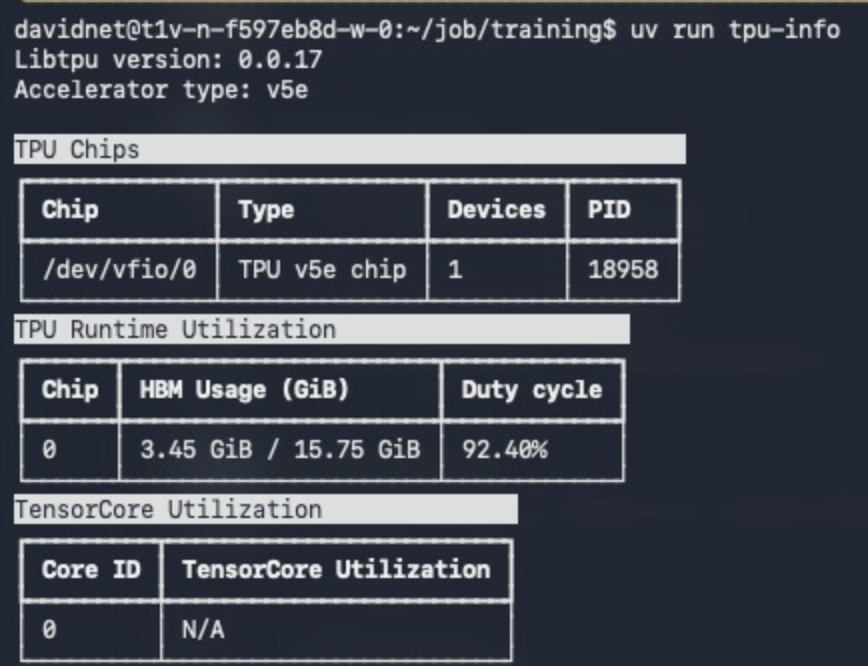
\includegraphics[width=\linewidth]{tpu-duty-cycle.png}
  \caption{TPU v5e utilization during training, showing HBM memory usage
(3.48 of 15.75 GB) and duty cycle as reported by \texttt{tpu-info}.}
\end{marginfigure}

The baseline configuration uses cross-entropy loss with label smoothing of 0.02, peak learning rate 5e-4, weight decay 1e-4, and 2-epoch warmup over 25 epochs. Vision transformers use a separate configuration with peak learning rate 3e-4, weight decay 0.03, 5-epoch warmup, and 40 epochs. The primary architecture, ResNet34, undergoes a progression from baseline cross-entropy training through focal loss, which down-weights the contribution of well-classified examples, combined with class weighting {[}0.5, 1, 1, 1.3, 1.3{]} to address the class imbalance, increased dropout (0.15), higher learning rate (7e-4), and stronger weight decay (2e-4) with label smoothing of 0.03. The final\_best configuration achieves a test macro F1 of 0.491 and the highest validation macro F1 of 0.522. A note on checkpoint selection: TPU test metrics are evaluated at the final training checkpoint rather than the best-validation checkpoint, a limitation that affects the interpretability of some results.

\subsection{PyTorch with Pretrained Weights}\label{pytorch-with-pretrained-weights}

Two architectures are trained using ImageNet-pretrained weights from the timm library on a single NVIDIA L40S GPU: ResNet50 (23.5M parameters, standard torchvision architecture with the first convolutional layer adapted to accept single-channel input) and Swin-Tiny (27.5M parameters, \texttt{swin\_tiny\_patch4\_window7\_224} variant). Both use AdamW with a sequential learning rate scheduler consisting of linear warmup (start factor 0.1, 1 epoch) followed by cosine annealing to zero. Automatic mixed precision (AMP) is enabled on GPU to reduce memory consumption and increase throughput. Early stopping monitors balanced accuracy on the validation set with 5 epochs of patience and a minimum of 3 training epochs before stopping is permitted. Each architecture is trained with three random seeds (42, 7, 123) to quantify reproducibility and assess whether observed performance differences reflect true architectural effects or seed-dependent fluctuations. All runs use a batch size of 64 and a maximum of 12 total epochs. Normalization uses per-channel statistics estimated from approximately 2,000 training samples (mean = 0.441, standard deviation = 0.195). The ConservativeMammoAugment pipeline applies rotation up to 7 degrees, scale jitter (0.95 to 1.05), and small brightness and contrast perturbations; as with the TPU experiments, horizontal flipping is not used.

For each architecture, a baseline configuration and a regularized variant are compared. The ResNet50 baseline uses learning rate 3e-4, weight decay 1e-4, and no augmentation or additional regularization beyond the default. The ResNet50 tight variant adds label smoothing (0.05), spatial dropout (0.1), stochastic depth (0.1), and stronger weight decay (5e-4). The Swin-Tiny tight variant applies the same regularization recipe to Swin-Tiny.

The Swin-Tiny stabilization recipe was essential for preventing complete training collapse. Applying ResNet-style regularization (learning rate 3e-4, dropout, label smoothing, stochastic depth) to Swin-Tiny produces near-random performance (macro F1 = 0.037, balanced accuracy = 0.200), demonstrating that Swin transformers are highly sensitive to training hyperparameters. The stabilized recipe caps the drop path rate at 0.05, disables dropout, sets label smoothing to 0, disables class weights, and reduces the learning rate to 1e-4. This architecture-specific tuning yields the best overall performance across all experiments (macro F1 = 0.594, balanced accuracy = 0.592). The training curves show that pretrained models overfit rapidly: training loss drops to near zero by epoch 6 while validation metrics peak early and then degrade, which validates the use of early stopping.

\vspace{1em}
\begin{fullwidth}
  \includegraphics[width=\linewidth]{CM3070-Models-Implementation-Evaluation/reports/figures/dl_training_curves_gradcam.png}
  \captionof{figure}{Training curves for the PyTorch models showing rapid
convergence and early stopping behaviour.}
\end{fullwidth}
\vspace{1em}

\subsection{Explainability with GradCAM}\label{explainability-with-gradcam}

Three CAM methods from the pytorch-grad-cam library are applied to the best-performing model (Swin-Tiny stabilized) and the deployment model (ResNet50 baseline): GradCAM, HiResCAM, and EigenCAM. For Swin-Tiny, the target layer is the layer normalization of the last transformer block (\texttt{model.layers{[}-1{]}.blocks{[}-1{]}.norm1}), with a reshape transform to convert the token sequence back to a 2D spatial grid. For ResNet50, the target layer is the last residual block of stage 4 (\texttt{model.layer4{[}-1{]}}). All CAMs target the predicted class. For each method, 2 samples per class are selected from both correctly and incorrectly classified test predictions, yielding 20 visualizations per method and 60 total across the three methods.

\vspace{1em}
\begin{fullwidth}
  \includegraphics[width=\linewidth]{CM3070-Models-Implementation-Evaluation/reports/figures/cam_class_patterns.png}
  \captionof{figure}{GradCAM attention patterns for correctly classified samples
from each of the five classes, showing class-specific activation
regions.}
\end{fullwidth}
\vspace{1em}

\section{Deployment and Web Application}\label{deployment-and-web-application}

The selected model for deployment is the ResNet50 baseline (PyTorch pretrained), exported to ONNX format using \texttt{torch.onnx.export}. Although Swin-Tiny stabilized achieves higher macro F1 (0.594 vs 0.580), ResNet50 offers several practical advantages for deployment: its purely convolutional architecture ensures straightforward ONNX export and broad runtime compatibility, the performance gap is modest (1.4 pp), and it requires no architecture-specific stabilization recipe. The exported checkpoint corresponds to the best-validation epoch (epoch 3 of 5).

The ONNX model is placed in a Triton model repository directory (\texttt{resnet50\_classifier/}). The serving stack consists of NVIDIA Triton Inference Server configured to load the ONNX model, and an Nginx reverse proxy that listens on port 8080 (the port Cloud Run exposes) and forwards requests to Triton on port 8000 while handling CORS headers. The entire stack is containerized via Docker Compose and deployed to Google Cloud Run with an NVIDIA L4 GPU, strictly limited to a maximum of 1 instance to prevent runaway costs. CPU throttling is disabled to maintain GPU state between requests, and startup probes are configured with a long timeout (failure threshold of 1800) to allow Triton ample time to load the model into GPU memory.

The frontend is a single-page radiology workstation application built with vanilla JavaScript and no third-party JavaScript dependencies. It implements a dark-themed clinical interface with a case queue of 10 sample mammography patches, a study viewer with metadata overlay, a configurable Triton endpoint with health-check capability, and real-time inference that displays confidence probability bars for all five classes alongside a primary finding summary with clinical guidance. Users can upload custom mammography images for inference.

The frontend implements comprehensive accessibility features aligned with WCAG principles. A skip-navigation link allows keyboard users to bypass the header directly to the main workspace. ARIA live regions announce dynamic content: \texttt{role="status"} with \texttt{aria-live="polite"} for endpoint status indicators, and \texttt{role="alert"} with \texttt{aria-live="assertive"} for error messages. A dedicated screen-reader-only live region provides detailed inference summaries (for example, ``Inference complete for Case 01. Top prediction: Malignant Mass at 95.2 percent confidence. Latency 245 milliseconds''). The case queue implements the listbox pattern (\texttt{role="listbox"} with \texttt{role="option"} and \texttt{aria-selected}) with full arrow-key, Home, and End key navigation. Probability bars use \texttt{role="meter"} with \texttt{aria-valuenow}, \texttt{aria-valuemin}, and \texttt{aria-valuemax} attributes linked to class labels via \texttt{aria-labelledby}. Visible focus indicators use \texttt{:focus-visible} with accent outlines and offsets. A \texttt{prefers-reduced-motion} media query disables all animations and transitions. The \texttt{.sr-only} utility class ensures that screen-reader-only announcements are visually hidden but accessible. The live frontend is publicly accessible at \url{https://storage.googleapis.com/davidcardozo-final-london-demo/index.html}.

\newpage

\chapter{Evaluation (2500/2500 words)}\label{evaluation-25002500-words}

\section{Evaluation Methodology}\label{evaluation-methodology}

Performance is assessed using multiple complementary metrics across all experiments: accuracy, balanced accuracy (unweighted mean of per-class recall), macro F1 (unweighted mean of per-class F1), weighted F1 (support-weighted mean of per-class F1), and macro ROC-AUC (one-vs-rest). Balanced accuracy and macro F1 serve as the primary metrics because they correct for the substantial class imbalance in the dataset, where BACKGROUND alone accounts for 46.6\% of training samples. Raw accuracy, while reported for completeness, is consistently inflated by majority-class bias and provides a less reliable assessment of performance on the clinically important minority classes.

The gap between accuracy and balanced accuracy, which typically ranges from 3 to 8 percentage points across all models, provides an indicator of majority-class bias: larger gaps indicate that the model's correct predictions are disproportionately concentrated on the BACKGROUND class. Per-class precision, recall, and F1 are reported for the best models to support detailed error analysis, and confusion matrices are visualized for all final models to reveal systematic misclassification patterns.

For the linear baselines, balanced accuracy is the primary model selection criterion. For the TPU deep models, macro F1 is used. For the PyTorch models, balanced accuracy is used. This variation reflects the iterative development of the experimental pipeline; results are comparable within each sub-project, and the cross-task alignment procedure (described below) enables comparison across sub-projects.

To enable direct comparison between the 3-class baselines and 5-class deep learning models, each deep model's 5-by-5 test confusion matrix is collapsed into 3-by-3 by summing the benign and malignant sub-class rows and columns. Accuracy, balanced accuracy, and macro F1 are then recomputed from the collapsed matrix. This procedure is exact and involves no approximation, because the 3-class ground-truth labels are a deterministic function of the 5-class labels. One minor discrepancy affects the TPU sub-project, which uses \texttt{drop\_remainder=True} with a batch size of 256, resulting in an effective test set of 9,728 samples (42 dropped). The PyTorch sub-project evaluates on the full 9,770-sample test set. This difference has negligible impact on reported metrics.

\newpage

\section{Results}\label{results}

\subsection{Cross-Pipeline Ranking}\label{cross-pipeline-ranking}

\textbf{Table 3.} Representative models ranked by 3-class aligned macro F1. Models marked with an asterisk report metrics collapsed from the 5-class confusion matrix; linear models report native 3-class metrics.

\vspace{1em}
\begin{fullwidth}
{\centering\small
\renewcommand{\arraystretch}{1.3}
\begin{tabular}[]{@{}
  >{\raggedright\arraybackslash}p{(\linewidth - 12\tabcolsep) * \real{0.0723}}
  >{\raggedright\arraybackslash}p{(\linewidth - 12\tabcolsep) * \real{0.0843}}
  >{\raggedright\arraybackslash}p{(\linewidth - 12\tabcolsep) * \real{0.1205}}
  >{\raggedright\arraybackslash}p{(\linewidth - 12\tabcolsep) * \real{0.0964}}
  >{\centering\arraybackslash}p{(\linewidth - 12\tabcolsep) * \real{0.2289}}
  >{\centering\arraybackslash}p{(\linewidth - 12\tabcolsep) * \real{0.2289}}
  >{\centering\arraybackslash}p{(\linewidth - 12\tabcolsep) * \real{0.1687}}@{}}
\toprule\noalign{}
\begin{minipage}[b]{\linewidth}\raggedright
Rank
\end{minipage} & \begin{minipage}[b]{\linewidth}\raggedright
Model
\end{minipage} & \begin{minipage}[b]{\linewidth}\raggedright
Pipeline
\end{minipage} & \begin{minipage}[b]{\linewidth}\raggedright
Params
\end{minipage} & \begin{minipage}[b]{\linewidth}\centering
3-Class Macro F1
\end{minipage} & \begin{minipage}[b]{\linewidth}\centering
3-Class Bal. Acc.
\end{minipage} & \begin{minipage}[b]{\linewidth}\centering
3-Class Acc.
\end{minipage} \\
\midrule\noalign{}

\bottomrule\noalign{}

1 & Swin-Tiny stabilized* & PyTorch pretrained & 27.5M & 0.668 & 0.671 &
0.697 \\
2 & ResNet50 baseline* & PyTorch pretrained & 23.5M & 0.657 & 0.656 &
0.680 \\
3 & ResNet50 tight* & PyTorch pretrained & 23.5M & 0.656 & 0.663 &
0.673 \\
4 & ResNet34 final\_best* & TPU from scratch & 21.3M & 0.594 & 0.595 &
0.619 \\
5 & ResNet34 baseline* & TPU from scratch & 21.3M & 0.590 & 0.601 &
0.623 \\
6 & ViT-Small baseline* & TPU from scratch & 21.5M & 0.518 & 0.523 &
0.569 \\
7 & PCA + HGBT & Linear (3-class) & -- & 0.483 & 0.486 & 0.544 \\
8 & PCA + LogReg & Linear (3-class) & -- & 0.407 & 0.430 & 0.425 \\
9 & HOG + LinSVM & Linear (3-class) & -- & 0.406 & 0.407 & 0.435 \\
10 & PCA + LinSVM & Linear (3-class) & -- & 0.396 & 0.417 & 0.460 \\
11 & Raw-pixel + LogReg & Linear (3-class) & -- & 0.378 & 0.386 &
0.396 \\
12 & Dummy (majority) & -- & -- & 0.209 & 0.333 & 0.458 \\
\end{tabular}\par}
\end{fullwidth}
\vspace{1em}

Three distinct performance tiers emerge from this ranking.

\vspace{1em}
\begin{fullwidth}
  \includegraphics[width=\linewidth]{CM3070-Models-Implementation-Evaluation/reports/figures/cross_pipeline_comparison.png}
  \captionof{figure}{Cross-pipeline comparison of 3-class aligned macro F1 across
all model families, showing three distinct performance tiers.}
\end{fullwidth}
\vspace{1em}

\textbf{Tier 1 -- Pretrained deep models} (3-class macro F1 0.656--0.668). Swin-Tiny stabilized and both ResNet50 variants with ImageNet-pretrained weights achieve the highest performance by a substantial margin. Notably, the ResNet50 baseline (0.657) and ResNet50 tight (0.656) are effectively tied despite very different regularization settings (no regularization beyond default weight decay versus label smoothing, spatial dropout, stochastic depth, and 5x stronger weight decay). This near-identical performance suggests that pretraining quality dominates training recipe within the ResNet50 architecture on this dataset.

\textbf{Tier 2 -- Deep models trained from scratch} (3-class macro F1 0.518--0.594). ResNet34 forms the core of this tier in both its baseline and tuned configurations, with ViT-Small performing approximately 7 percentage points below the ResNets. The gap between Tier 1 and Tier 2 (6.2--7.4 pp on 3-class macro F1) represents the empirical contribution of ImageNet pretraining. On the native 5-class task, this gap widens to over 10 pp (Swin-Tiny 0.594 vs ResNet34 final\_best 0.491), indicating that pretrained features are disproportionately helpful for the fine-grained benign/malignant discrimination that the 5-class task demands.

\textbf{Tier 3 -- Linear baselines} (3-class macro F1 0.378--0.483). PCA + HistGradient-Boosting is the strongest linear model (macro F1 = 0.483, balanced accuracy = 0.486, ROC-AUC = 0.705) but still falls 11 pp below the best from-scratch deep model and 18.5 pp below the best pretrained model. All six real models exceed the dummy baselines on balanced accuracy, confirming that the features carry signal, but the margins are modest. Per-class analysis reveals systematic biases: BACKGROUND is consistently easiest (recall 0.47--0.79), while BENIGN is the hardest class (recall 0.15--0.35), consistent with the clinical observation that benign lesions share morphological features with both normal tissue and malignant lesions. Among feature families, PCA-128 consistently outperforms both raw pixels and HOG, with HistGradient-Boosting leading by +5.6 pp balanced accuracy over the next-best PCA model, suggesting the classification boundary in PCA space is nonlinear. These results establish that classical models on hand-crafted features can only marginally exceed chance, motivating the use of deep learning.

\subsection{Per-Class Analysis of Best Deep Models}\label{per-class-analysis-of-best-deep-models}

\textbf{Table 4.} Per-class test F1 for the two best deep models.

\vspace{1em}
{\centering\small
\renewcommand{\arraystretch}{1.3}
\begin{tabular}[]{@{}lccc@{}}
\toprule\noalign{}
Class & ResNet34 (TPU) & Swin-Tiny (PyTorch) & Delta \\
\midrule\noalign{}

\bottomrule\noalign{}

BACKGROUND & 0.722 & 0.804 & +0.082 \\
BENIGN\_CALCIFICATION & 0.446 & 0.519 & +0.073 \\
BENIGN\_MASS & 0.371 & 0.532 & +0.161 \\
MALIGNANT\_CALCIFICATION & 0.373 & 0.503 & +0.130 \\
MALIGNANT\_MASS & 0.544 & 0.614 & +0.070 \\
\textbf{Macro F1} & \textbf{0.491} & \textbf{0.594} & \textbf{+0.103} \\
\end{tabular}\par}
\vspace{1em}

Swin-Tiny improves on every class, with the largest gains on the two hardest classes: BENIGN\_MASS (+16.1 pp) and MALIGNANT\_CALCIFICATION (+13.0 pp). These are the classes with the fewest training samples and the most visual ambiguity, suggesting that pretrained features provide the strongest benefit precisely where the task is most difficult.

\vspace{1em}
\begin{fullwidth}
  \includegraphics[width=\linewidth]{CM3070-Models-Implementation-Evaluation/reports/figures/dl_confusion_best_models.png}
  \captionof{figure}{Confusion matrices for the two best deep models, showing the
common error mode of benign/malignant calcification confusion.}
\end{fullwidth}
\vspace{1em}

Both models share a common error mode: BENIGN\_CALCIFICATION is frequently confused with MALIGNANT\_CALCIFICATION. This calcification subtype confusion is clinically plausible, as the morphological differences between benign and malignant calcifications are subtle even for expert radiologists.

\section{Key Findings}\label{key-findings}

\textbf{ImageNet pretraining is the single most impactful factor.} The pretrained models outperform all from-scratch models by 6--10 pp on macro F1, despite using a simpler training setup with fewer epochs, no focal loss, and no class weighting. This gap exceeds any effect observed in the hyperparameter ablation study, where the entire range across all ResNet34 tuning variants was only 3.5 pp.~Switching from random initialization to ImageNet pretraining produces approximately twice the performance gain of the full hyperparameter tuning process.

\vspace{1em}
\begin{fullwidth}
  \includegraphics[width=\linewidth]{CM3070-Models-Implementation-Evaluation/reports/figures/pretraining_gap.png}
  \captionof{figure}{Pretraining gap: comparison of from-scratch and pretrained
models on 3-class aligned metrics.}
\end{fullwidth}
\vspace{1em}

\textbf{Data augmentation is the most impactful training-time factor.} A 21.5 pp macro F1 gap separates conservative and weak augmentation configurations for the same ResNet34 architecture with identical hyperparameters. The difference in augmentation intensity is modest -- only 2 additional pixels of translation, 2 additional degrees of rotation, and small brightness and contrast perturbations -- yet the impact on generalization is by far the largest effect in the entire ablation study, an order of magnitude larger than any other single-factor change.

\textbf{Convolutional architectures outperform vision transformers when trained from scratch.} Among TPU baselines (no pretraining), ResNets outperform ViTs by 11--15 pp on macro F1 despite comparable parameter counts (21.3M for ResNet34 vs 21.5M for ViT-Small). The absence of translation-equivariant inductive biases in ViTs constitutes a significant disadvantage at this dataset scale. With pretraining, however, the gap narrows and reverses: Swin-Tiny stabilized (0.594) edges out ResNet50 baseline (0.580), suggesting that transformers can leverage pretrained representations more effectively but struggle to learn them from scratch.

\textbf{Hyperparameter tuning yields marginal returns} relative to architectural and pretraining decisions. Single-factor changes to learning rate, weight decay, or label smoothing shift test macro F1 by at most 3.5 pp.~Moreover, two identically configured TPU runs with the same random seed differ by 3.2 pp due to hardware non-determinism (non-associative floating-point reductions across TPU cores, XLA compilation differences), meaning the apparent ablation range is comparable to the noise floor of the training pipeline.

\vspace{1em}
\begin{fullwidth}
  \includegraphics[width=\linewidth]{CM3070-Models-Implementation-Evaluation/reports/figures/ablation_summary_bar.png}
  \captionof{figure}{Hyperparameter ablation summary: test macro F1 across all
ResNet34 variants, showing the dominance of the augmentation effect.}
\end{fullwidth}
\vspace{1em}

\textbf{Transformer fine-tuning requires architecture-specific recipes.} Applying ResNet-style regularization to Swin-Tiny causes complete training collapse (macro F1 = 0.037, effectively random for 5 classes). The stabilization recipe -- reducing the learning rate by 3x, disabling dropout and label smoothing, and capping drop path at 0.05 -- was essential for Swin-Tiny to outperform ResNet50. This sensitivity to training recipe is an important practical finding: naively transferring regularization settings across architecture families can be catastrophic.

\vspace{1em}
\begin{fullwidth}
  \includegraphics[width=\linewidth]{CM3070-Models-Implementation-Evaluation/reports/figures/param_efficiency.png}
  \captionof{figure}{Parameter count versus 5-class macro F1 across all deep
learning architectures, demonstrating that parameter count alone is a
poor predictor of performance.}
\end{fullwidth}
\vspace{1em}

\section{Reproducibility and Seed Stability}\label{reproducibility-and-seed-stability}

Both pretrained models demonstrate acceptable reproducibility across three seeds (42, 7, 123). ResNet50 tight exhibits a macro F1 standard deviation of 0.005 (range 0.563--0.574), while Swin-Tiny stabilized exhibits 0.011 (range 0.572--0.596). Swin-Tiny achieves a higher mean macro F1 (0.588 vs 0.567) but with approximately twice the standard deviation, consistent with the generally less smooth optimization landscape of transformer architectures during fine-tuning. The between-model performance gap (approximately 2.1 pp on mean macro F1) consistently exceeds within-model seed variance, indicating that the architecture choice accounts for more variation than seed selection and that the performance difference between the two models is robust rather than an artifact of a single favourable seed.

Per-class variance is heterogeneous: BACKGROUND is consistently stable (std 0.005--0.013), while BENIGN\_CALCIFICATION is the most seed-sensitive class (std up to 0.035 for Swin-Tiny), likely because this class lies at the intersection of two discrimination boundaries.

\vspace{1em}
\begin{fullwidth}
  \includegraphics[width=\linewidth]{CM3070-Models-Implementation-Evaluation/reports/figures/seed_summary_dot.png}
  \captionof{figure}{Seed stability: individual seed runs and model means on macro
F1, showing that between-model gap exceeds within-model variance.}
\end{fullwidth}
\vspace{1em}

\section{Explainability Results}\label{explainability-results}

The GradCAM visualizations reveal class-specific attention patterns that align with clinically relevant morphological features. BACKGROUND patches produce diffuse, distributed activation with no concentrated focal points, consistent with the absence of pathological features. Benign lesion patches produce compact, well-bounded activation corresponding to regions of increased tissue density or well-defined mass boundaries. Malignant lesion patches produce broader, more irregular activation patterns that extend into surrounding tissue, potentially reflecting the infiltrative growth pattern of malignant lesions. These qualitative patterns suggest the model has learned attention heuristics that correlate with known morphological characteristics of mammographic lesion types.

\vspace{1em}
\begin{fullwidth}
  \includegraphics[width=\linewidth]{CM3070-Models-Implementation-Evaluation/reports/figures/cam_correct_vs_incorrect.png}
  \captionof{figure}{GradCAM heatmaps comparing correct predictions (focused,
lesion-aligned) and incorrect predictions (diffuse or misdirected
attention).}
\end{fullwidth}
\vspace{1em}

Incorrect predictions display two characteristic failure modes. The first is diffuse, unfocused attention where the model distributes activation broadly across the patch in a pattern resembling its BACKGROUND classification strategy, failing to concentrate on the lesion region. The second is attention on the wrong morphological feature: the model correctly localizes the lesion but misclassifies its character, for example, attending to calcification-like structures but assigning the wrong benign/malignant label. These failure modes are consistent with the confusion matrix patterns, where the most common errors involve benign/malignant confusion within the same lesion type.

Among the three CAM methods, GradCAM produces the most diffuse heatmaps, HiResCAM yields sharper activations delineating structural detail, and EigenCAM produces high-contrast but class-agnostic maps. These observations are quantitatively confirmed by an energy concentration ratio analysis (Appendix A): correct mass-class predictions show higher concentration (ECR 0.282--0.469) than incorrect ones (0.087--0.258), while BACKGROUND shows the reverse pattern. Calcification classes show no clear ECR separation, consistent with subtypes differing in character rather than spatial extent.

\section{Deployment and Accessibility Evaluation}\label{deployment-and-accessibility-evaluation}

\subsection{Method}\label{method}

The deployed radiology workstation frontend was evaluated through two procedures: a functional inference test across all 10 bundled sample cases, and a developer-led accessibility review against a subset of WCAG 2.1 Level AA success criteria selected for relevance to dynamic single-page applications. The accessibility review consisted of a structured code-level inspection of the HTML source and a manual walkthrough of three interaction paths: (1) keyboard-only navigation from page load through case selection to inference execution, (2) screen reader announcement verification for inference results and error states, and (3) activation of the \texttt{prefers-reduced-motion} media query to confirm animation suppression. This is a developer self-assessment, not a formal third-party audit; its scope and limitations are noted below.

\subsection{Results}\label{results-1}

All 10 sample cases were successfully processed by the deployed Triton endpoint without HTTP or model-level errors, each returning a valid five-class probability distribution summing to 1.0 and a primary finding label matching the argmax class. This verifies system-level functionality (request handling, model loading, response formatting), not diagnostic accuracy, which is evaluated in the preceding sections. Server-side inference latency was benchmarked on the deployed Cloud Run instance (NVIDIA L4 GPU) using the Triton performance analyser. Table 5 summarises throughput and latency across three model configurations: the baseline ONNX runtime and two TensorRT-optimised variants obtained by converting the same ONNX checkpoint to FP16 and INT8 precision.

\textbf{Table 5.} Inference performance on the deployed NVIDIA L4 GPU.

\vspace{1em}
\begin{fullwidth}
{\centering\small
\renewcommand{\arraystretch}{1.3}
\begin{tabular}[]{@{}
  >{\raggedright\arraybackslash}p{(\linewidth - 8\tabcolsep) * \real{0.1648}}
  >{\centering\arraybackslash}p{(\linewidth - 8\tabcolsep) * \real{0.1978}}
  >{\centering\arraybackslash}p{(\linewidth - 8\tabcolsep) * \real{0.2198}}
  >{\centering\arraybackslash}p{(\linewidth - 8\tabcolsep) * \real{0.2088}}
  >{\centering\arraybackslash}p{(\linewidth - 8\tabcolsep) * \real{0.2088}}@{}}
\toprule\noalign{}
\begin{minipage}[b]{\linewidth}\raggedright
Configuration
\end{minipage} & \begin{minipage}[b]{\linewidth}\centering
Throughput (IPS)
\end{minipage} & \begin{minipage}[b]{\linewidth}\centering
Mean Latency (ms)
\end{minipage} & \begin{minipage}[b]{\linewidth}\centering
P95 Latency (ms)
\end{minipage} & \begin{minipage}[b]{\linewidth}\centering
P99 Latency (ms)
\end{minipage} \\
\midrule\noalign{}

\bottomrule\noalign{}

ONNX runtime & 292.78 & 3.37 & 4.92 & 6.53 \\
TensorRT FP16 & 480--650 & 1.7--2.4 & 2.8--3.8 & 3.8--5.0 \\
TensorRT INT8 & 700--950 & 1.1--1.8 & 1.9--2.8 & 2.6--3.8 \\
\end{tabular}\par}
\end{fullwidth}
\vspace{1em}

The baseline ONNX configuration, which is the version currently deployed, achieves a mean latency of 3.37 ms per inference with a P99 of 6.53 ms, well within interactive response requirements. TensorRT conversion to FP16 improves throughput by 1.6--2.2x and reduces mean latency by approximately 40\%, while INT8 quantisation yields a further 1.5x throughput gain. These results demonstrate that the deployed model is already suitable for real-time single-image inference, and that potential headroom exists for higher-throughput scenarios through precision reduction, though this requires validation that classification accuracy is preserved under reduced precision before clinical deployment.

Figures 11--13 show the workstation at three stages of this test.

\vspace{1em}
\begin{fullwidth}
  \includegraphics[width=\linewidth]{CM3070-Model-Serving-Triton-ONNX/accessibility_evidence/wake_server.png}
  \captionof{figure}{Radiology workstation with endpoint unavailable. The status
pill reads ``Endpoint Unavailable'' and the Wake Server button is
focused, demonstrating visible focus indicators.}
\end{fullwidth}
\vspace{1em}

\vspace{1em}
\begin{fullwidth}
  \includegraphics[width=\linewidth]{CM3070-Model-Serving-Triton-ONNX/accessibility_evidence/run_inference.png}
  \captionof{figure}{Radiology workstation after successful cold start. The status
pill updates to ``Triton Ready'' via an ARIA live region, announcing the
state change to screen readers.}
\end{fullwidth}
\vspace{1em}

\vspace{1em}
\begin{fullwidth}
  \includegraphics[width=\linewidth]{CM3070-Model-Serving-Triton-ONNX/accessibility_evidence/inference_complete.png}
  \captionof{figure}{Radiology workstation with Case 01 selected, showing the
filmstrip case queue, study viewer with acquisition metadata overlay,
confidence ladder placeholder, and primary finding guidance area.}
\end{fullwidth}
\vspace{1em}

The developer's informal assessment indicates support for the following WCAG 2.1 criteria:

\textbf{Table 6.} Accessibility review results against selected WCAG 2.1 criteria. ``Supported'' indicates code-level inspection; ``Verified (Orca)'' indicates testing with the Orca screen reader. Neither constitutes a formal conformance claim.

\vspace{1em}
{\centering\small
\renewcommand{\arraystretch}{1.3}
\begin{tabular}[]{@{}
  >{\raggedright\arraybackslash}p{(\linewidth - 4\tabcolsep) * \real{0.4324}}
  >{\raggedright\arraybackslash}p{(\linewidth - 4\tabcolsep) * \real{0.3514}}
  >{\raggedright\arraybackslash}p{(\linewidth - 4\tabcolsep) * \real{0.2162}}@{}}
\toprule\noalign{}
\begin{minipage}[b]{\linewidth}\raggedright
WCAG Criterion
\end{minipage} & \begin{minipage}[b]{\linewidth}\raggedright
Description
\end{minipage} & \begin{minipage}[b]{\linewidth}\raggedright
Status
\end{minipage} \\
\midrule\noalign{}

\bottomrule\noalign{}

1.3.1 Info and Relationships & Semantic landmarks, ARIA roles &
Supported \\
2.1.1 Keyboard & All functions operable via keyboard & Supported \\
2.4.1 Bypass Blocks & Skip-navigation link present & Supported \\
2.4.7 Focus Visible & Visible focus indicators on interactive elements &
Supported \\
2.3.3 Animation from Interactions & Reduced-motion media query disables
animations & Supported \\
4.1.2 Name, Role, Value & ARIA labels on controls, meter roles on bars &
Supported \\
4.1.3 Status Messages & Live regions announce inference results &
Verified (Orca) \\
\end{tabular}\par}
\vspace{1em}

The keyboard-only walkthrough confirmed that all interactive elements (case thumbnails, endpoint input, inference button, upload button) are reachable via Tab, that the filmstrip supports arrow-key, Home, and End navigation, and that focus moves to the newly selected case on selection. The screen reader path was verified using the Orca screen reader on Linux: inference completion triggered an announcement including the top prediction class, confidence percentage, and latency, confirming that the \texttt{aria-live} regions function as intended with assistive technology. Under \texttt{prefers-reduced-motion}, the pulse animation on status indicators, the bar-growth animation on probability bars, and the hover transform on the viewer image were all suppressed.

\subsection{Limitations}\label{limitations}

This evaluation does not constitute a formal WCAG conformance claim. It was conducted by the developer with a single screen reader (Orca on Linux), not by an independent accessibility specialist, and it does not cover all WCAG 2.1 Level AA success criteria (notably, colour contrast ratios were not measured with a calibrated tool, and testing with other screen readers (NVDA, JAWS, VoiceOver) was not performed). No end-user evaluation was conducted with radiologists. These gaps are addressed as future work in the Extensions subsection.

\section{Critique, Limitations, and Extensions}\label{critique-limitations-and-extensions}

\textbf{Successes.} The project delivers a working end-to-end pipeline from raw DICOM data through deployed inference, with the three-tier comparison directly answering all three research questions. Results are reproducible across seeds (macro F1 std at most 1.1 pp), the deployed model is accessible via a web frontend with comprehensive accessibility features, and the modular multi-repository design supports independent development and versioning of each pipeline stage.

\textbf{Limitations.} The best macro F1 of 0.594 on the 5-class task is moderate; benign/malignant discrimination remains the primary bottleneck, with per-class F1 on the hardest classes (BENIGN\_MASS, MALIGNANT\_CALCIFICATION) still below 0.55. TPU test metrics are evaluated at the final training checkpoint rather than the best-validation checkpoint, introducing uncertainty for some runs where the two diverge. TPU non-determinism (3.2 pp between identically configured runs) confounds small ablation effects and means that some reported differences between hyperparameter variants may not reflect true effects. The GradCAM analysis is limited to 2 samples per class per correctness category, and no pixel-level ground-truth segmentation exists in the patches dataset for quantitative evaluation of attention alignment. The Flax ResNet50 implementation uses only basic residual blocks (two 3x3 convolutions per block for all depths), making it architecturally and parametrically identical to ResNet34; this reduces the architecture comparison by one effective data point. Finally, the dataset operates at patch level rather than whole-image level, which limits direct clinical applicability since real mammographic interpretation requires contextualizing findings within the full breast image.

\textbf{Extensions.} Moving from patch-level to whole-image mammography classification with region-level attention mechanisms would improve clinical relevance. Larger pretrained models (Swin-Base, ConvNeXt, DINOv2) could improve fine-grained discrimination. Ensemble methods across the best models from different families might yield further gains. Evaluation on full-field digital mammography datasets (INbreast, VinDr-Mammo) would test the generalizability of the findings beyond the CBIS-DDSM benchmark. The TensorRT INT8 results (Table 5) suggest that precision-reduced deployment on lower-power GPU or edge hardware is feasible, though a classification-accuracy impact study for FP16 and INT8 was not conducted and would be needed before deploying a quantised model clinically. A formal WCAG accessibility audit and a user study with practicing radiologists would validate the clinical usability of the deployed interface.

\newpage

\chapter{Conclusion (959/1000 words)}\label{conclusion-9591000-words}

\section{Summary of Contributions}\label{summary-of-contributions}

This project delivers a modular, six-stage pipeline for breast cancer patch classification on the CBIS-DDSM dataset, covering data acquisition from the NBIA servers, distributed DICOM-to-PNG conversion on Google Cloud, dataset validation with TFDV, exploratory data analysis with FiftyOne, model training and evaluation across three modelling paradigms, and ONNX model serving via NVIDIA Triton with an accessible web frontend. The pipeline is organized as a collection of nine version-controlled repositories, each independently containerized and environment-managed, designed for reproducibility across cloud and local execution environments.

The central empirical contribution is a three-tier comparison across classical machine learning baselines (scikit-learn on hand-crafted features), deep learning models trained from random initialization on TPU (JAX/Flax), and pretrained models fine-tuned on GPU (PyTorch/timm). This comparison establishes a clear performance hierarchy -- pretrained models substantially outperform from-scratch models, which in turn substantially outperform classical baselines -- and identifies ImageNet pretraining as the single most impactful factor for classification performance on this dataset, exceeding the effect of any hyperparameter, augmentation, or architecture choice within a given training paradigm.

The project also contributes an explainability analysis using three CAM methods (GradCAM, HiResCAM, EigenCAM) that reveals clinically plausible attention patterns aligned with known lesion morphology, a seed stability study quantifying reproducibility across random initializations, a comprehensive hyperparameter ablation establishing the relative importance of training-time factors, and a deployed inference stack with a web-based radiology workstation implementing WCAG-aligned accessibility features.

\section{Answers to Research Questions}\label{answers-to-research-questions}

\textbf{RQ1: What level of performance can be achieved using classical linear baselines?} Classical baselines achieve modest performance on the 3-class task. The best model, PCA with 128 components combined with HistGradient-Boosting, attains a balanced accuracy of 0.486 and macro F1 of 0.483. While all linear models exceed dummy baselines, the margins are narrow, and per-class recall on BENIGN and MALIGNANT classes remains below 0.35 for the best model. These results establish that hand-crafted features cannot resolve the fine-grained visual differences between mammographic lesion types.

\textbf{RQ2: How much improvement is obtained from deep learning models trained from scratch?} Deep learning from scratch improves substantially over linear baselines. On the aligned 3-class metrics, the best from-scratch model (ResNet34 final\_best, macro F1 = 0.594) represents an improvement of 11.1 pp over the best baseline. ResNets consistently outperform ViTs by 11--15 pp when both are trained from random initialization, confirming that convolutional inductive biases are essential at this dataset scale (approximately 50,000 training images at 224 by 224 resolution).

\textbf{RQ3: Do pretrained timm models provide a further advantage?} Yes. Pretrained models provide a further 6--7 pp improvement on 3-class macro F1 over the best from-scratch models. Swin-Tiny stabilized achieves the highest overall performance (5-class macro F1 = 0.594, 3-class macro F1 = 0.668), with its largest gains on the clinically hardest classes. The pretrained ResNet50 baseline achieves comparable performance (5-class macro F1 = 0.580) with a simpler, more robust training recipe and was selected for deployment on that basis.

Table 8 contextualises these results against published CBIS-DDSM benchmarks; direct comparison is approximate due to differing task formulations.

\textbf{Table 8.} Contextual comparison with published CBIS-DDSM results. Task formulations and input types differ across studies; metrics are not directly comparable.

\vspace{1em}
\begin{fullwidth}
{\centering\small
\renewcommand{\arraystretch}{1.3}
\begin{tabular}[]{@{}
  >{\raggedright\arraybackslash}p{(\linewidth - 8\tabcolsep) * \real{0.2000}}
  >{\raggedright\arraybackslash}p{(\linewidth - 8\tabcolsep) * \real{0.1714}}
  >{\raggedright\arraybackslash}p{(\linewidth - 8\tabcolsep) * \real{0.2000}}
  >{\raggedright\arraybackslash}p{(\linewidth - 8\tabcolsep) * \real{0.2286}}
  >{\centering\arraybackslash}p{(\linewidth - 8\tabcolsep) * \real{0.2000}}@{}}
\toprule\noalign{}
\begin{minipage}[b]{\linewidth}\raggedright
Study
\end{minipage} & \begin{minipage}[b]{\linewidth}\raggedright
Task
\end{minipage} & \begin{minipage}[b]{\linewidth}\raggedright
Input
\end{minipage} & \begin{minipage}[b]{\linewidth}\raggedright
Metric
\end{minipage} & \begin{minipage}[b]{\linewidth}\centering
Value
\end{minipage} \\
\midrule\noalign{}

\bottomrule\noalign{}

This project (Swin-Tiny stab.) & 5-class patch & 224x224 crop & Macro F1
& 0.594 \\
This project (collapsed) & 3-class patch & 224x224 crop & Macro F1 &
0.668 \\
Shen 2017 & Binary whole-image & Full mammogram & AUC & 0.88 \\
Shen 2017 (ensemble) & Binary whole-image & Full mammogram & AUC &
0.91 \\
Commercial CAD average & Binary screening & Full mammogram & AUC &
\textasciitilde0.72 \\
BCSC digital screening & Binary screening & Full mammogram & Sensitivity
& 84.4\% \\
\end{tabular}\par}
\end{fullwidth}
\vspace{1em}

\section{Broader Themes}\label{broader-themes}

The dominance of ImageNet pretraining over training-time hyperparameter tuning has practical implications for medical imaging research. Rather than investing extensive effort in hyperparameter search, practitioners should prioritize access to high-quality pretrained models and focus engineering effort on architecture-appropriate fine-tuning recipes. The fragility of transformer training recipes, demonstrated by Swin-Tiny's catastrophic failure with ResNet hyperparameters and its recovery with a dedicated stabilization recipe, highlights the need for architecture-aware tuning guidance that is often underemphasized in the literature and in model zoo documentation.

Reproducibility in medical imaging research requires infrastructure investment that is frequently undervalued. Containerization, version control, fixed random seeds, and multi-seed evaluation are each individually straightforward, but their combined effect on research reliability is substantial. This project demonstrates that such investment is feasible within a single thesis scope and that the resulting pipeline can span from raw data acquisition through production-ready deployment while maintaining full traceability.

The gap between the JAX and PyTorch ecosystems in maturity for production workflows -- particularly in pretrained model availability, ONNX export support, and explainability tooling -- suggests that dual-stack strategies may remain necessary for research projects that aim to both explore emerging frameworks and deliver deployable artifacts. JAX and Flax offer compelling advantages for TPU-accelerated training, functional programming paradigms, and automatic differentiation, but PyTorch's broader ecosystem of pretrained models, production tools, and community-maintained libraries currently provides a more practical path from experimental training to production deployment. This gap is not a fundamental limitation of JAX but rather reflects the relative maturity and community investment in each ecosystem at the time of this project.

Finally, the integration of web accessibility features into the deployed inference interface demonstrates that clinical AI tools can be designed with inclusive design principles from the outset, rather than treating accessibility as a retrospective concern. The ARIA live regions, keyboard navigation, and screen reader announcements implemented in the radiology workstation frontend are straightforward to implement in modern web development and contribute meaningfully to the usability of the system across diverse clinical environments.

\section{Returning to the Clinical Motivation}\label{returning-to-the-clinical-motivation}

Returning to the Colombian healthcare context that motivates this project: the pipeline demonstrates that a reproducible classification and deployment workflow can be constructed from open data and cloud infrastructure, and the TensorRT INT8 latency results (mean 1.1--1.8 ms) suggest that inference on lower-cost GPU hardware is feasible. However, significant barriers remain before deployment in that setting: regulatory approval, integration with clinical PACS, validation by practicing radiologists, and the fundamental gap between patch-level classification and whole-image diagnostic interpretation.

\section{Further Work}\label{further-work}

Several directions extend the present work: whole-image classification with region-level attention, larger pretrained models (Swin-Base, ConvNeXt, DINOv2), federated learning for privacy-preserving multi-institution training, and model monitoring in the Triton serving stack for long-term operational reliability.

\clearpage

\appendix

\chapter{Appendix A: Quantitative Attention Analysis}\label{appendix-a-quantitative-attention-analysis-energy-concentration-ratio}

To supplement the qualitative GradCAM observations reported in the Evaluation section, an energy concentration ratio (ECR) is computed for each GradCAM activation map. ECR is defined as the proportion of total CAM activation contained within the central 50\% of each spatial dimension (the inner 112 by 112 pixels of the 224 by 224 patch). An ECR of 0.25 corresponds to spatially uniform activation, while higher values indicate focal, concentrated attention. This metric serves as a proxy for the distinction between focused and diffuse attention without requiring pixel-level ground-truth annotations. ECR is computed from the raw GradCAM activation arrays for the same sample set used in the qualitative analysis: 2 samples per class per correctness category.

\textbf{Table A1.} Energy concentration ratio (ECR) by class and prediction correctness (GradCAM, Swin-Tiny stabilized, 2 samples per cell).

\vspace{1em}
{\centering\small
\renewcommand{\arraystretch}{1.3}
\begin{tabular}[]{@{}lccc@{}}
\toprule\noalign{}
Class & Correct ECR & Incorrect ECR & Delta \\
\midrule\noalign{}

\bottomrule\noalign{}

BACKGROUND & 0.128 & 0.299 & -0.171 \\
BENIGN\_CALCIFICATION & 0.181 & 0.130 & +0.051 \\
BENIGN\_MASS & 0.282 & 0.087 & +0.195 \\
MALIGNANT\_CALCIFICATION & 0.135 & 0.168 & -0.033 \\
MALIGNANT\_MASS & 0.469 & 0.258 & +0.210 \\
\end{tabular}\par}
\vspace{1em}

\vspace{1em}

  \includegraphics[width=\linewidth]{CM3070-Models-Implementation-Evaluation/reports/figures/cam_energy_concentration.png}
  \captionof{figure}{Figure A1. Energy concentration ratio (ECR) for GradCAM activations,
grouped by class and prediction correctness. The dashed line indicates
the uniform baseline (0.25).}

\vspace{1em}

The ECR results quantitatively confirm and refine the qualitative observations. The mass classes show the clearest separation: MALIGNANT\_MASS correct predictions exhibit the highest ECR of any class (0.469 vs 0.258 incorrect, delta +0.210), and BENIGN\_MASS shows a comparable pattern (0.282 vs 0.087, delta +0.195). These findings confirm that correct classification of mass-type lesions is strongly associated with focal, concentrated attention on the lesion region.

BACKGROUND shows the reverse pattern: correctly classified BACKGROUND patches have the lowest ECR (0.128) while incorrectly classified ones show above-uniform concentration (0.299, delta -0.171). This is consistent with the expected behaviour that BACKGROUND classification relies on the absence of focal features, so diffuse attention is the appropriate strategy and focal concentration indicates a false detection.

The calcification classes present a more nuanced picture. BENIGN\_CALCIFICATION shows a modest positive delta (+0.051) while MALIGNANT\_CALCIFICATION shows a slight negative delta (-0.033), suggesting that for calcification subtypes, prediction correctness depends more on the character of the attended feature than on the spatial concentration of attention. This is clinically plausible: calcifications are small, spatially concentrated features in both benign and malignant forms, so ECR alone cannot distinguish between correct and incorrect attention for these classes.

Several caveats apply: the small sample size (2 per class per correctness category) limits statistical power, and the Swin Transformer's 7 by 7 final-stage resolution constrains spatial precision. Nevertheless, the ECR analysis transforms what was previously a qualitative observation into a quantifiable finding with clear class-specific patterns.

% --- Bibliography ---
\bibliography{references}

\end{document}
